\documentclass[a4paper,11pt]{article}
\usepackage[utf8]{inputenc}
\usepackage[T1]{fontenc}
\usepackage[english]{babel}
\usepackage[margin=1.5cm]{geometry} 
\usepackage{graphicx}
\usepackage{subcaption}
\usepackage{float}
\usepackage{parskip}
\usepackage{caption}
\usepackage{fontawesome5}
\usepackage{amsmath}
\usepackage{amssymb}
\usepackage{xcolor}
\usepackage[linesnumbered, ruled, vlined]{algorithm2e}
\SetKwInput{Input}{Input}
\SetKwInput{Output}{Output}
\SetKw{ReturnKw}{return}
\SetKwFor{ForEachLoop}{for each}{do}{end}
\SetKwFor{ForLoop}{for}{do}{end}
\SetKwIF{IfCond}{ElseIfCond}{ElseCond}{if}{then}{else}{else if}{end}
\SetKw{UpTo}{to}
\SetKw{RepeatKw}{repeat}
\SetKw{WhileKw}{while}
\SetKwRepeat{RepeatUntil}{repeat}{until}
\newcommand{\Call}[2]{\textsc{#1}(#2)}

\title{\vspace{-2cm} \textbf{An Algorithm on Thin Walls}}
\author{Marco Busetti}
\date{\today}

\begin{document}

\maketitle
\thispagestyle{empty}

\section*{Introduction}
This mini-report presents some visual results obtained in thin wall identification simulations for various geometries, along with the algorithms responsible for the method.

Some clarifications:

\begin{itemize}
    \item \textbf{White edges:} outline of the outer polygon;
    \item \textbf{Yellow edges:} outlines of the polygon's holes;
    \item \textbf{Green edges:} medial axis of the geometry;
    \item \textbf{Colored-area polygons:} polygons that represent the thin wall regions (the polygons).
\end{itemize}

\newpage

\section*{Spurious Branch Filtering}

The first step in identifying thin walls is filtering the spurious branches of the straight skeleton of the polygon of the evaluated slice. 

The spurious branch filtering problem is critical for thin wall analysis because it allows the removal of noise and original branches of the straight skeleton that are not part of the analysis for identifying thin walls and that do not correspond to the expected mechanical outcome of printing the part. 

An algorithm that handles the filtering of spurious branches of a part through a topological and geometric procedure is proposed below. 

Note that the spurious branch filtering problem may have different outputs depending on the user's intent. For a given part, the user may be interested in keeping or removing certain regions that can be considered spurious branches. This requires the introduction of a variable, the ``Pruning Threshold $L_{prune}$'', which corresponds to a multiple of the threshold established for classifying thin wall regions. That is: 

\[
L_{prune} = k\cdot T_{max}, \; k\in\mathbb{R}_{\geq 0}
\]

Where $T_{max}$ represents the maximum diameter of the inscribed circle for the region to be classified as thin. 

 \begin{algorithm}[H]

\caption{Filter Spurious Branches}

\label{alg:filter_spurious_balanced}

\Input{Straight Skeleton $S$, Pruning Threshold $L_{prune}$.}
\Output{Set of edges to remove $A_{rem}$.}

$A_{rem} \leftarrow \{e \in S.edges \mid e$ connects a boundary vertex to a skeleton vertex$\}$\;

\RepeatUntil{$changed = \text{false}$}{
    $Items \leftarrow \emptyset$\;

    \ForEachLoop{skeleton vertex $v$}{
        $g \leftarrow \Call{EffectiveDegree}{v, A_{rem}}$\;

        \IfCond{$g \geq 3$}{
            \ForEachLoop{edge $e$ incident to $v$ with $e \notin A_{rem}$}{
                $C \leftarrow$ path that starts at $v$ along $e$ and continues through vertices of effective degree 2\;
                \IfCond{$C$ ends at a leaf \textbf{and} every vertex of $C$ is at a distance less than $L_{prune}$ from $v$}{
                    $Items \leftarrow Items \cup \{(v, C, d_{max}, \text{false})\}$\;
                }
            }
        }

        \IfCond{$g = 1$}{
            $C \leftarrow$ path that starts at leaf $v$ and continues through vertices of effective degree 2\;
            \IfCond{$C$ ends at another leaf \textbf{and} every vertex of $C$ is at a distance less than $L_{prune}$ from $v$}{
                $Items \leftarrow Items \cup \{(v, C, d_{max}, \text{true})\}$\;
            }
        }
    }

    $\Call{SortAscending}{Items, d_{max}}$\;
    $changed \leftarrow \text{false}$\;

    \ForEachLoop{item $(v, C, d_{max}, island) \in Items$}{
        \IfCond{$C \cap A_{rem} = \emptyset$}{
            \IfCond{$island$ \textbf{or} $\Call{EffectiveDegree}{v, A_{rem} \cup C} \geq 1$}{
                $A_{rem} \leftarrow A_{rem} \cup C$\;
                $changed \leftarrow \text{true}$\;
            }
        }
    }
}

\ReturnKw $A_{rem}$\;

\end{algorithm} 

The idea of the algorithm above can be visualized with the following region of a given polygon:

\begin{figure}[H]
    \centering
    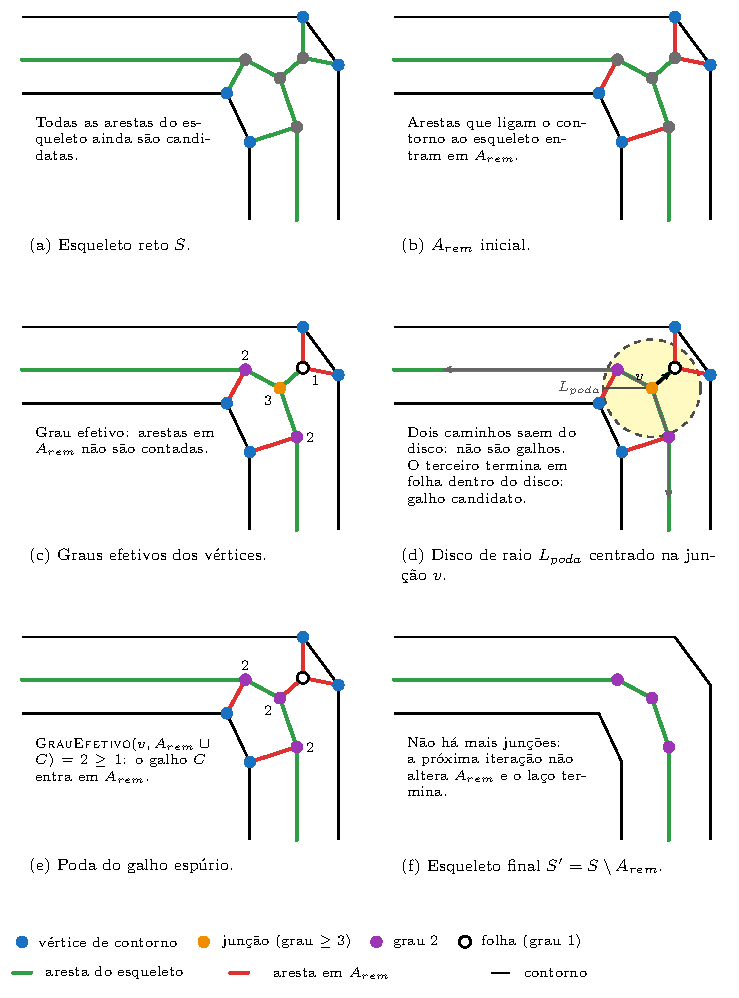
\includegraphics[width=0.85\textwidth]{imgs/visu.pdf}     
    \caption{Step-by-step execution of Algorithm~\ref{alg:filter_spurious_balanced} on a thin wall corner. The cut in (e) only occurs because the junction $v$ keeps an effective degree $\geq 1$ after the removal.}
\end{figure}

Below, some results of the filtered medial axis are presented for certain slices, with different values of $L_{prune}$ for a given constant value of $T_{max}$.

\begin{figure}[htbp]
    \centering
    \begin{subfigure}{0.32\textwidth}
        \centering
        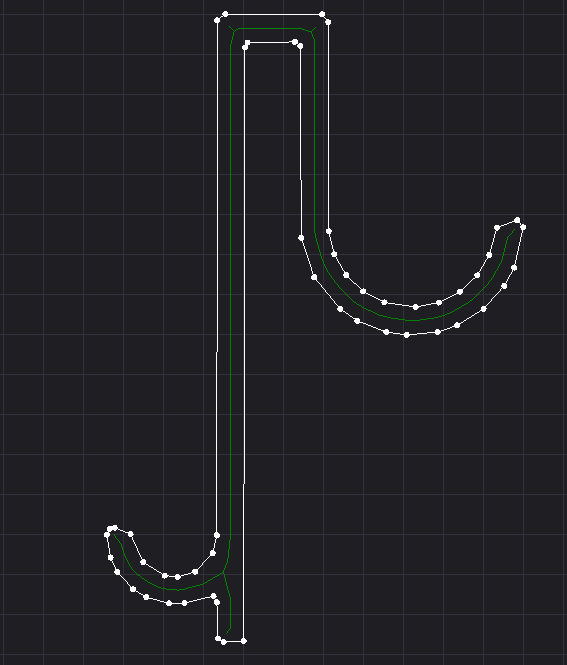
\includegraphics[width=\linewidth]{imgs/hook1.png}
        \caption{Hook geometry with \\$L_{prune} = 0\cdot T_{max}$}
        \label{fig:sub1}
    \end{subfigure}\hfill
    \begin{subfigure}{0.32\textwidth}
        \centering
        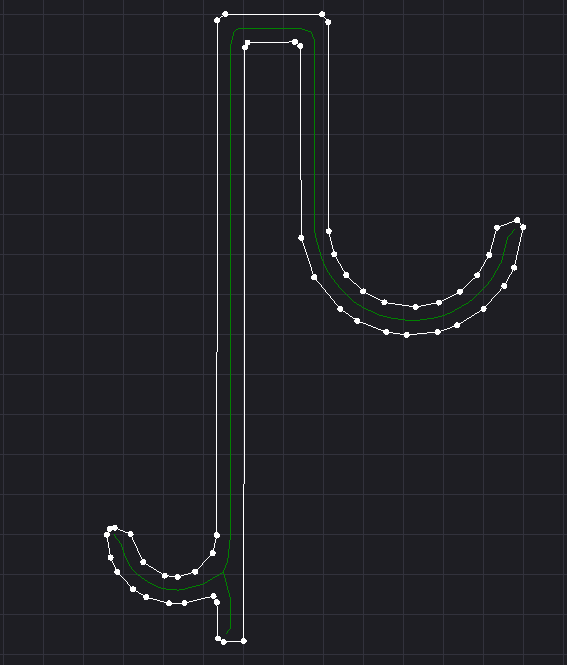
\includegraphics[width=\linewidth]{imgs/hook2.png}
        \caption{Hook geometry with \\$L_{prune} = 1\cdot T_{max}$}
        \label{fig:sub2}
    \end{subfigure}\hfill
    \begin{subfigure}{0.32\textwidth}
        \centering
        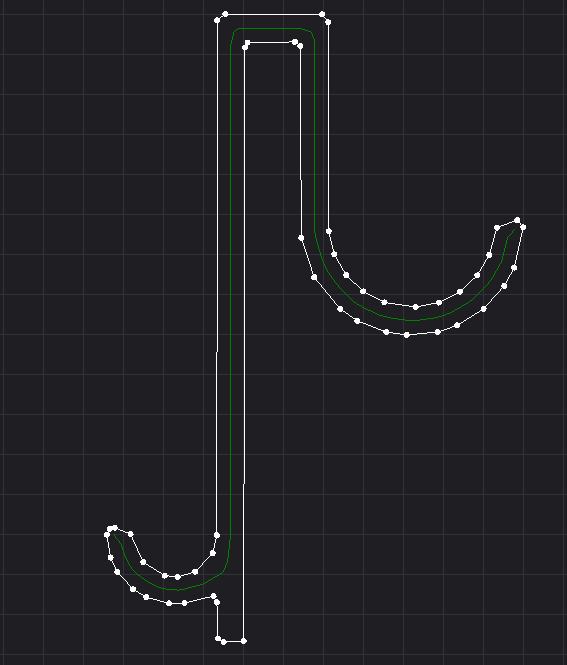
\includegraphics[width=\linewidth]{imgs/hook3.png}
        \caption{Hook geometry with \\$L_{prune} = 5\cdot T_{max}$}
        \label{fig:sub3}
    \end{subfigure}
    \label{fig:tres_imagens}
\end{figure}

\begin{figure}[htbp]
    \centering
    \begin{subfigure}{0.48\textwidth}
        \centering
        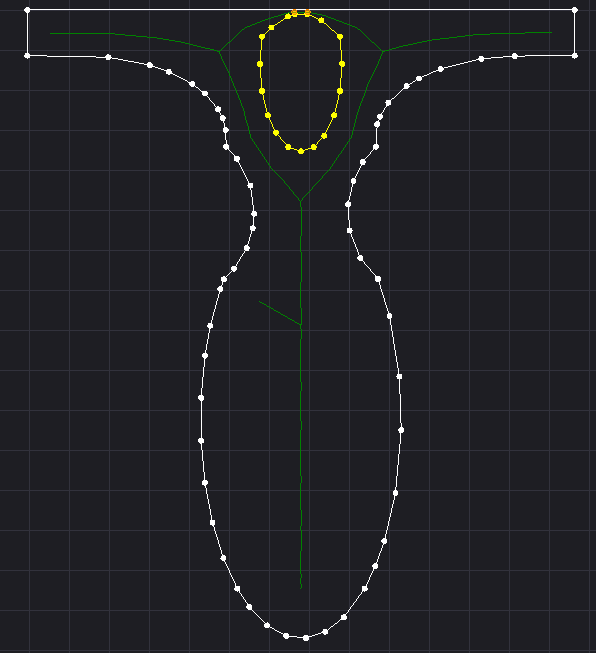
\includegraphics[width=\linewidth]{imgs/esoterico1.png}
        \caption{Coat rack geometry with \\
        $L_{prune}=0\cdot T_{max}$}
        \label{fig:sub1}
    \end{subfigure}\hfill
    \begin{subfigure}{0.48\textwidth}
        \centering
        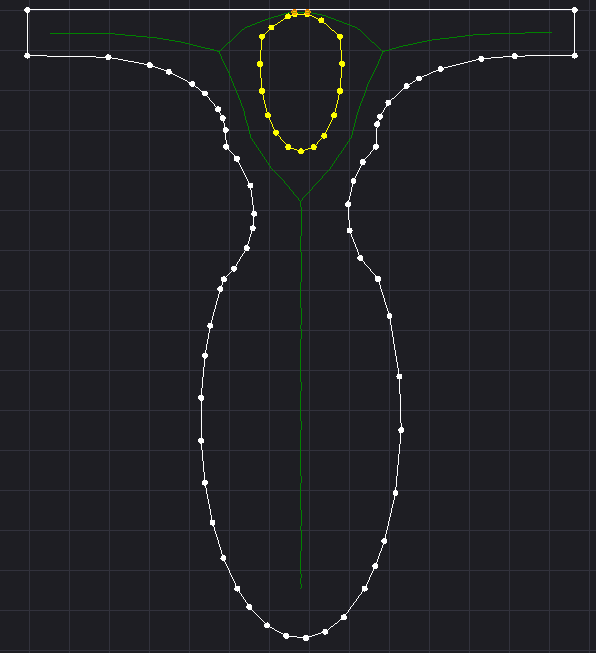
\includegraphics[width=\linewidth]{imgs/esoterico2.png}
        \caption{Coat rack geometry with \\
        $L_{prune}=10\cdot T_{max}$}
        \label{fig:sub2}
    \end{subfigure}
    \label{fig:duas_imagens}
\end{figure}

\begin{figure}[htbp]
    \centering
        \begin{subfigure}{0.48\textwidth}
        \centering
        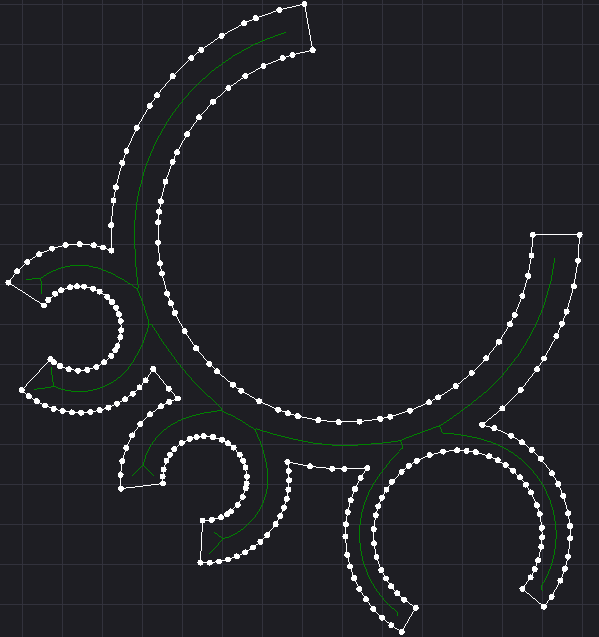
\includegraphics[width=\linewidth]{imgs/clamp1.png}
        \caption{Clamp geometry with \\
        $L_{prune}=0\cdot T_{max}$}
        \label{fig:sub1}
    \end{subfigure}\hfill
    \begin{subfigure}{0.48\textwidth}
        \centering
        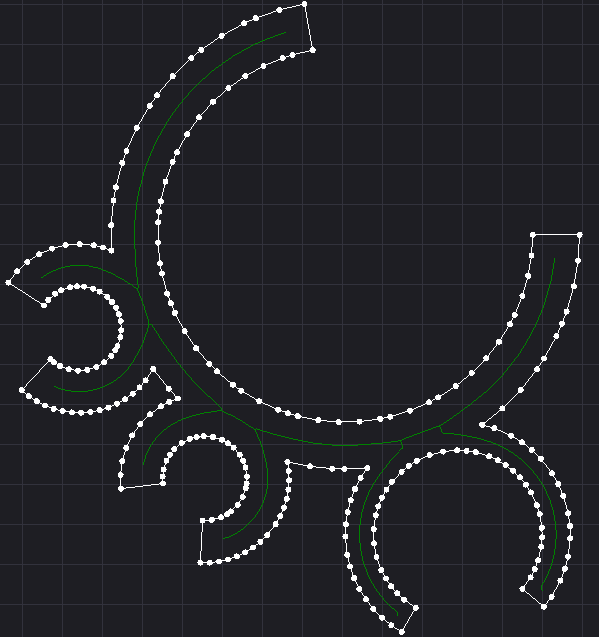
\includegraphics[width=\linewidth]{imgs/clamp2.png}
        \caption{Clamp geometry with \\
        $L_{prune}=5\cdot T_{max}$}
        \label{fig:sub2}
    \end{subfigure}
    
    \label{fig:duas_imagens}
\end{figure}

\begin{figure}[htbp]
    \centering
    
    \begin{subfigure}{0.48\textwidth}
        \centering
        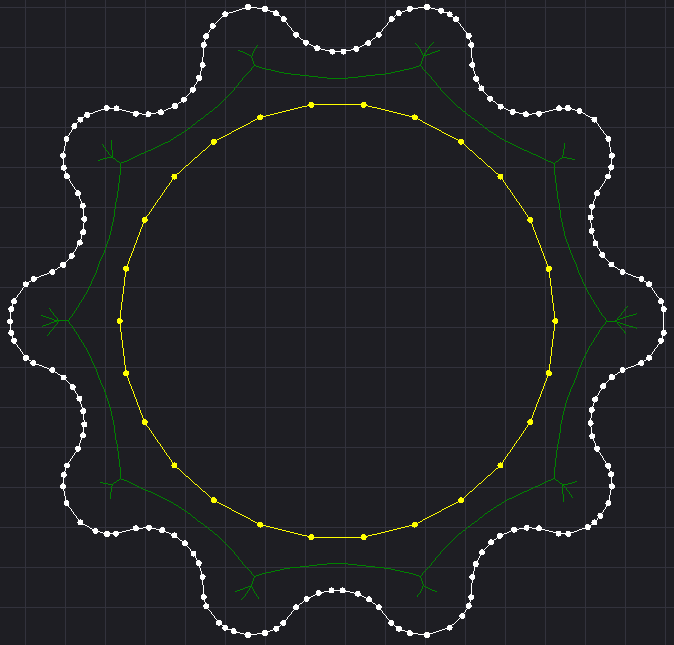
\includegraphics[width=\linewidth]{imgs/knobi1.png}
        \caption{Gear geometry with \\
        $L_{prune}=0\cdot T_{max}$}
        \label{fig:sub1}
    \end{subfigure}\hfill
    \begin{subfigure}{0.48\textwidth}
        \centering
        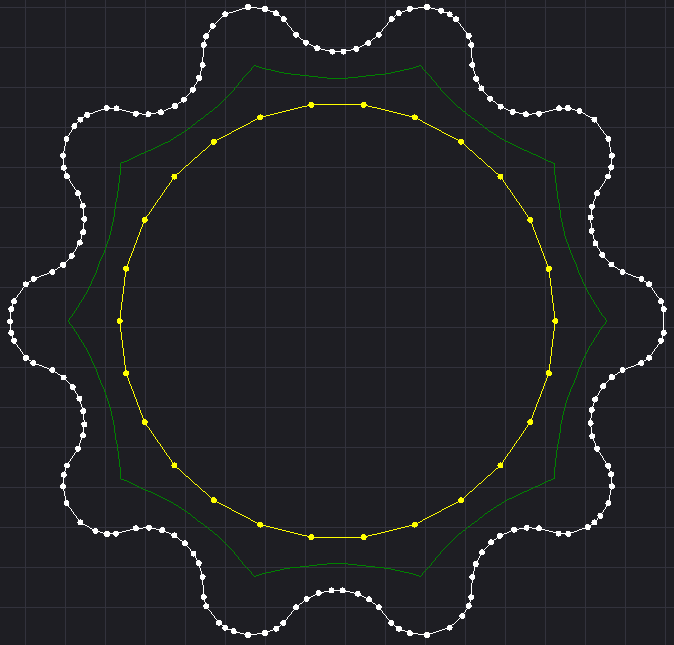
\includegraphics[width=\linewidth]{imgs/knobi2.png}
        \caption{Gear geometry with \\
        $L_{prune}=3\cdot T_{max}$}
        \label{fig:sub2}
    \end{subfigure}
    \label{fig:duas_imagens}
\end{figure}

\newpage

\section*{Thin Wall Identification}

After the spurious branch filtering step, we can proceed to the thin wall identification method and the construction of the respective thin wall polygons. The algorithm that handles this task is proposed below:

\begin{algorithm}[H]
\caption{Identify Thin Walls}
\label{alg:thinwall_chains}

\Input{Polygon $P$, Holes $H$, Maximum Thickness $T_{max}$, Pruning Factor $f_{prune}$.}
\Output{List of polygons with holes $\mathcal{U}_{walls}$.}

$\mathcal{L}_{chains} \leftarrow \emptyset$\;
$S \leftarrow \Call{BuildStraightSkeleton}{P, H}$\;
$L_{prune} \leftarrow f_{prune} \cdot T_{max}$\;
$A_{rem} \leftarrow \Call{FilterSpuriousBranches}{S, L_{prune}}$\;
$E_{medial} \leftarrow \Call{FilterMedialAxis}{S, A_{rem}}$\;

$Threshold \leftarrow T_{max} / 2.0$\;

\tcc{Find the parametric bounds $(t_0, t_1)$ of the thin segments}
$ThinSegments \leftarrow \emptyset$\;
\ForEachLoop{half-edge $he \in E_{medial}$}{
    $v_{src} \leftarrow he.origin, \quad v_{tgt} \leftarrow he.target$\;
    $t_{src} \leftarrow v_{src}.time, \quad t_{tgt} \leftarrow v_{tgt}.time$\;

    \IfCond{$t_{src} < Threshold$ \textbf{or} $t_{tgt} < Threshold$}{
        $[t_0, t_1] \leftarrow \Call{ComputeThresholdBounds}{t_{src}, t_{tgt}, Threshold}$\;
        \IfCond{$|t_1 - t_0| > \varepsilon$}{
            $ThinSegments[he] \leftarrow (he, t_0, t_1)$\;
            $ThinSegments[he.opposite] \leftarrow (he.opposite, 1-t_1, 1-t_0)$\;
        }
    }
}

\tcc{Build continuous chains of thin walls}
$V_{visited} \leftarrow \emptyset$\;
\ForEachLoop{half-edge $he_{base} \in E_{medial}$}{
    \IfCond{$he_{base} \in V_{visited}$ \textbf{or} $he_{base} \notin ThinSegments$}{
        \textbf{continue}\;
    }

    $Chain \leftarrow \Call{StartChain}{ThinSegments[he_{base}]}$\;
    $\Call{Mark}{V_{visited}, he_{base}}$\;

    \tcc{Grow forward: continues while the segment extends to the end of the edge, the target vertex has degree 2 in $S$, and the next segment is thin and unvisited}
    $Chain \leftarrow \Call{GrowChainForward}{Chain, ThinSegments, V_{visited}}$\;

    \tcc{Grow backward: analogous, starting from the beginning of the first segment}
    $Chain \leftarrow \Call{GrowChainBackward}{Chain, ThinSegments, V_{visited}}$\;

    $\Omega \leftarrow \Call{BuildChainPolygon}{Chain}$\;
    \IfCond{$\Omega \neq \emptyset$}{
        $\mathcal{L}_{chains} \leftarrow \mathcal{L}_{chains} \cup \{\Omega\}$\;
    }
}

\tcc{Unification of the thin walls}
$\mathcal{U}_{walls} \leftarrow \Call{ExactPolygonUnion}{\mathcal{L}_{chains}}$\;

\ReturnKw $\mathcal{U}_{walls}$\;
\end{algorithm}

\begin{algorithm}[H]
\caption{Build Chain Polygon}
\label{alg:cadeia_poligono}

\Input{Chain of thin segments $Chain = (c_1, \dots, c_n)$, where $c_i = (he_i, t_0^i, t_1^i)$.}
\Output{Thin wall polygon $\Omega$, or $\emptyset$ if the construction fails.}

\tcc{Chain endpoints on the medial axis}
$Q_{start} \leftarrow \Call{StartPoint}{c_1}$\;
$Q_{end} \leftarrow \Call{EndPoint}{c_n}$\;

\tcc{Projections onto the boundary edges that define the faces at the endpoints}
$Pl_{start} \leftarrow \Call{ProjectOntoBoundary}{Q_{start}, he_1}$\;
$Pr_{start} \leftarrow \Call{ProjectOntoBoundary}{Q_{start}, he_1.opposite}$\;
$Pl_{end} \leftarrow \Call{ProjectOntoBoundary}{Q_{end}, he_n}$\;
$Pr_{end} \leftarrow \Call{ProjectOntoBoundary}{Q_{end}, he_n.opposite}$\;
\IfCond{any projection fails}{
    \ReturnKw $\emptyset$\;
}

$BoundaryPoints \leftarrow \emptyset$\;

\tcc{Initial cap and left side (forward)}
$\Call{Add}{BoundaryPoints, Q_{start}}$\;
$\Call{Add}{BoundaryPoints, Pl_{start}}$\;
\ForLoop{$i \leftarrow 1$ \UpTo $n-1$}{
    $\Call{AddSharedVertex}{he_i, he_{i+1}, BoundaryPoints}$\;
}

\tcc{Final cap}
$\Call{Add}{BoundaryPoints, Pl_{end}}$\;
$\Call{Add}{BoundaryPoints, Q_{end}}$\;
$\Call{Add}{BoundaryPoints, Pr_{end}}$\;

\tcc{Right side (backward)}
\ForLoop{$i \leftarrow n$ \UpTo $2$ (decreasing)}{
    $\Call{AddSharedVertex}{he_i.opposite, he_{i-1}.opposite, BoundaryPoints}$\;
}
$\Call{Add}{BoundaryPoints, Pr_{start}}$\;

\tcc{Build and validate the polygon}
$\Omega \leftarrow \Call{CreatePolygon}{BoundaryPoints}$\;
\IfCond{$|\Omega| < 3$ \textbf{or} $\Omega$ is not simple}{
    \ReturnKw $\emptyset$\;
}
$\Call{OrientCounterclockwise}{\Omega}$\;

\ReturnKw $\Omega$\;
\end{algorithm}

Below, some tests performed for a given fixed $T_{max}$ and $L_{prune} = 2\cdot T_{max}$ are presented.

Two visualizations of the thin wall polygons are presented:
\begin{itemize}
    \item ``Chain'' visualization of polygons: this visualization results from the procedural stitching of the polygons during the iteration over the medial axis edges of the geometry. Each polygon ``chain'' is the stitching of all thin wall polygons of a region bounded by vertices of degree $\geq3$. The visual effect is several groups of polygons denoted by different colors;
    \item Unified Visualization: this visualization is the result of the union of all the polygon groups generated during the stitching. The visual effect is a single polygon group denoted by one color.
\end{itemize}


\subsection*{Cogwheel}
\vspace*{\fill}
\begin{figure}[H]
    \centering
    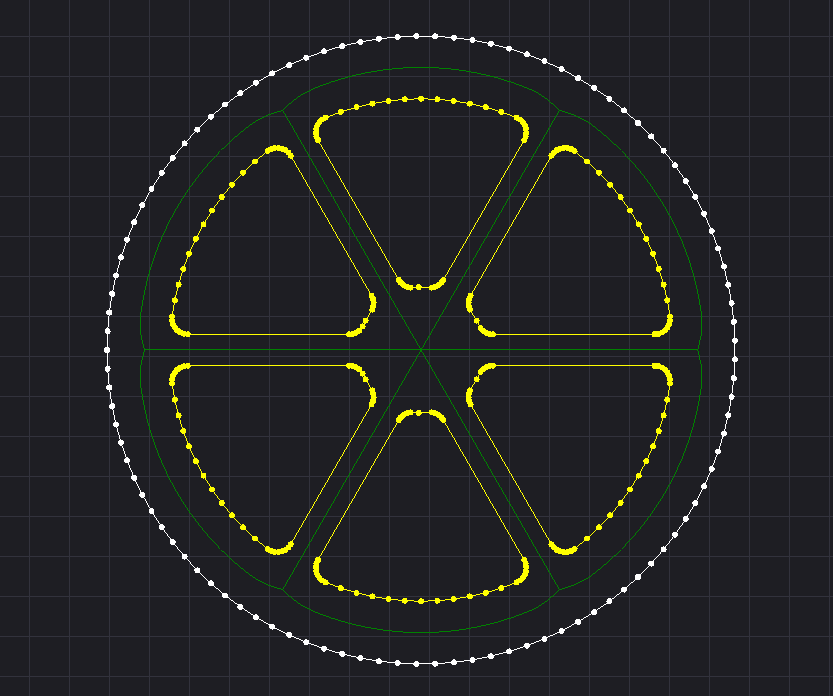
\includegraphics[width=0.85\textwidth]{imgs/roda.png} 
    \caption{Polygon for the Cogwheel}
\end{figure}
\vspace*{\fill}
\clearpage
\begin{figure}[H]
    \centering
    \begin{subfigure}{0.48\textwidth}
        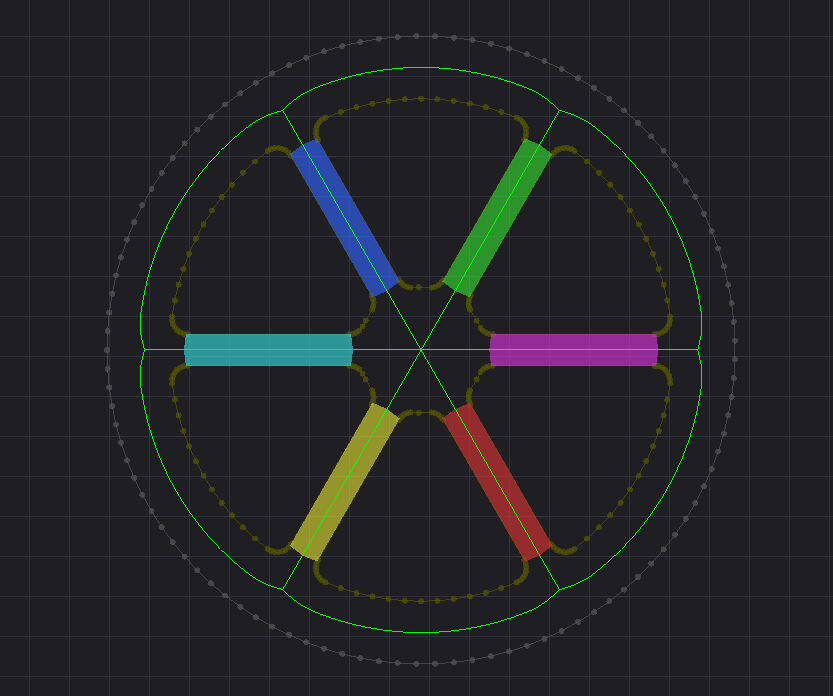
\includegraphics[width=\linewidth]{imgs/roda_ps.png}
        \caption{Thin Walls in groups with \textit{threshold $T_1$}}
    \end{subfigure}\hfill
    \begin{subfigure}{0.48\textwidth}
        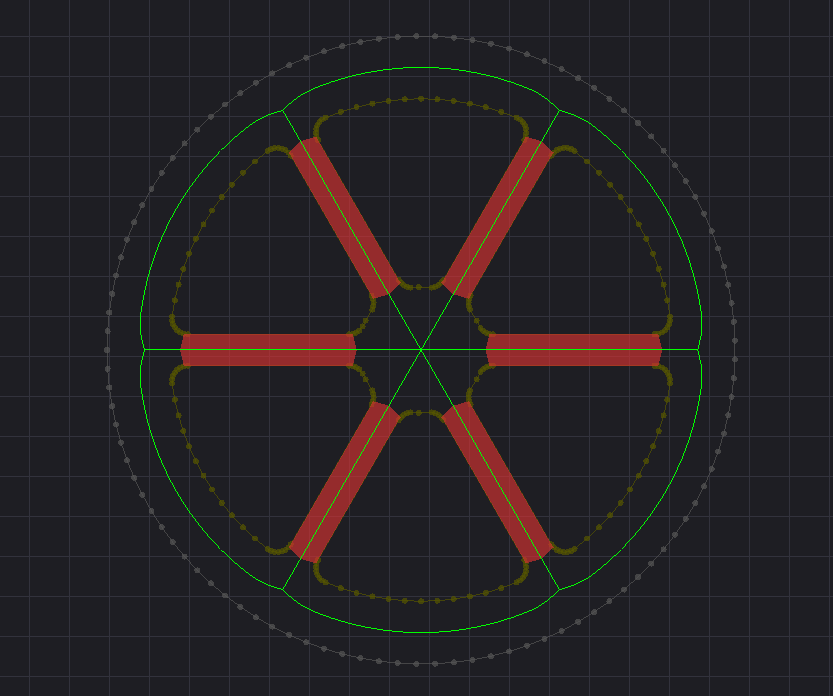
\includegraphics[width=\linewidth]{imgs/roda_pj.png}
        \caption{Merged Thin Walls with \textit{threshold $T_1$}}
    \end{subfigure}
    
    \vspace{0.3cm}
    
    \begin{subfigure}{0.48\textwidth}
        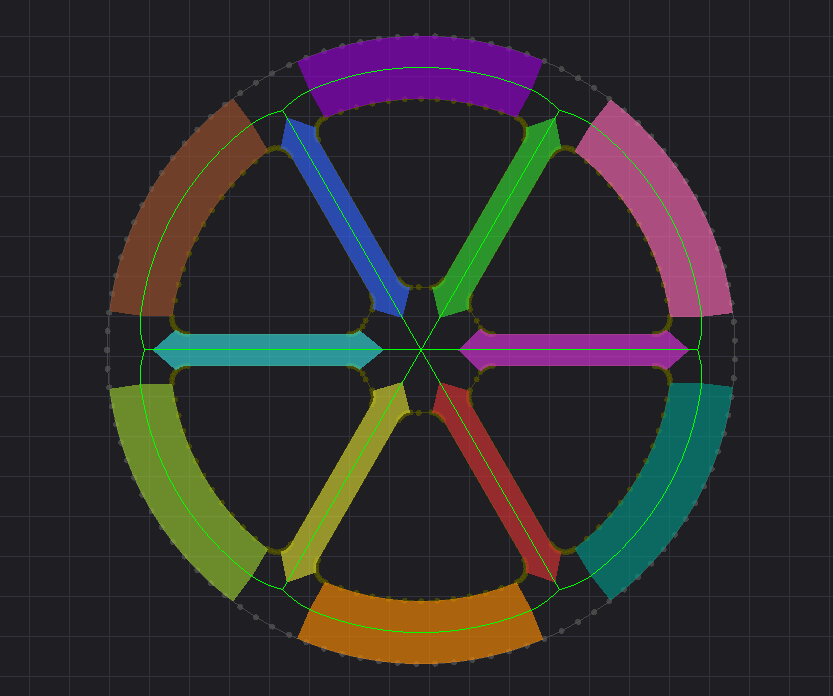
\includegraphics[width=\linewidth]{imgs/roda_ps2.png}
        \caption{Thin Walls in groups with \textit{threshold $T_2>T_1$}}
    \end{subfigure}\hfill
    \begin{subfigure}{0.48\textwidth}
        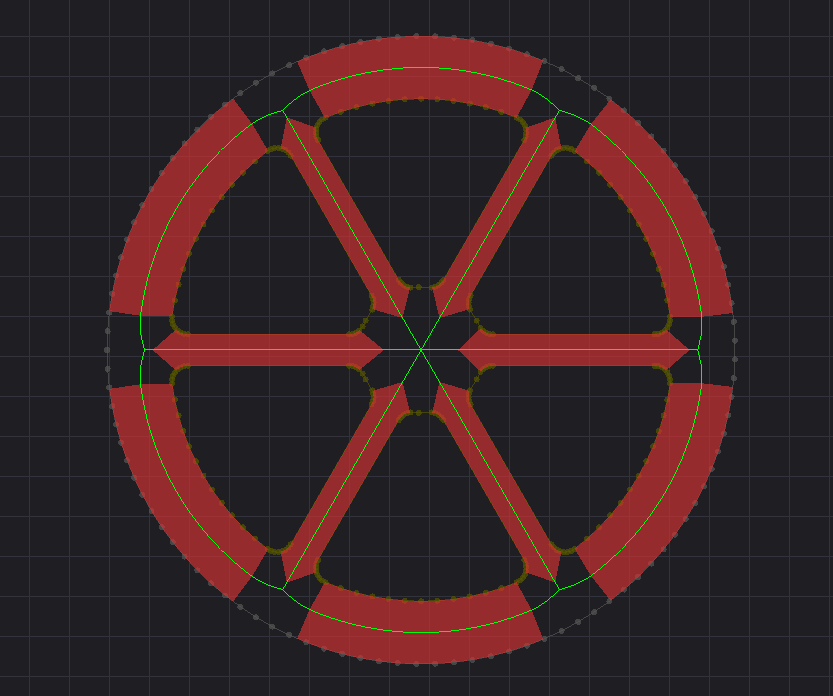
\includegraphics[width=\linewidth]{imgs/roda_pj2.png}
        \caption{Merged Thin Walls with \textit{threshold $T_2>T_1$}}
    \end{subfigure}
    
    \vspace{0.3cm}
    
    \begin{subfigure}{0.48\textwidth}
        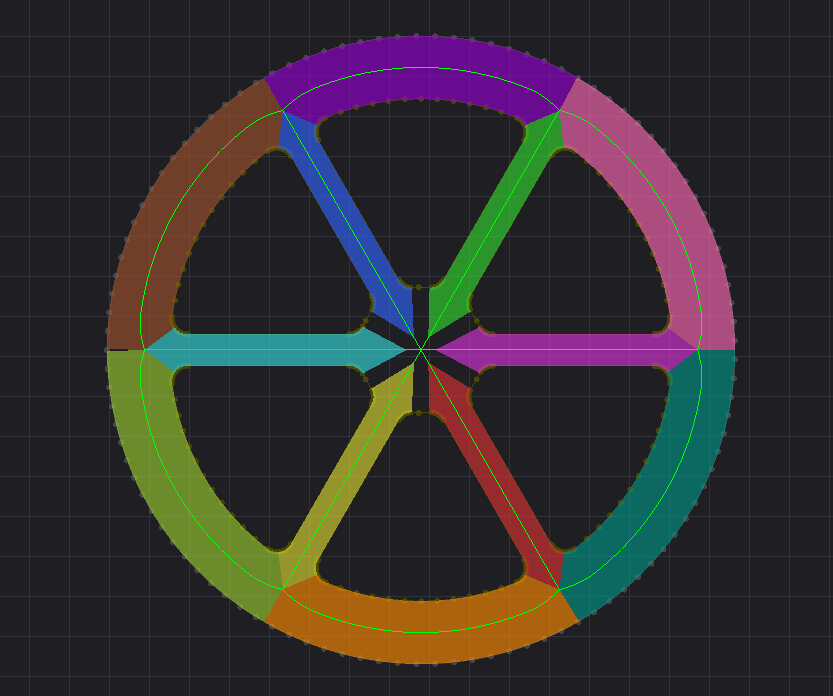
\includegraphics[width=\linewidth]{imgs/roda_ps3.png}
        \caption{Thin Walls in groups with \textit{threshold $T_3>T_2$}}
    \end{subfigure}\hfill
    \begin{subfigure}{0.48\textwidth}
        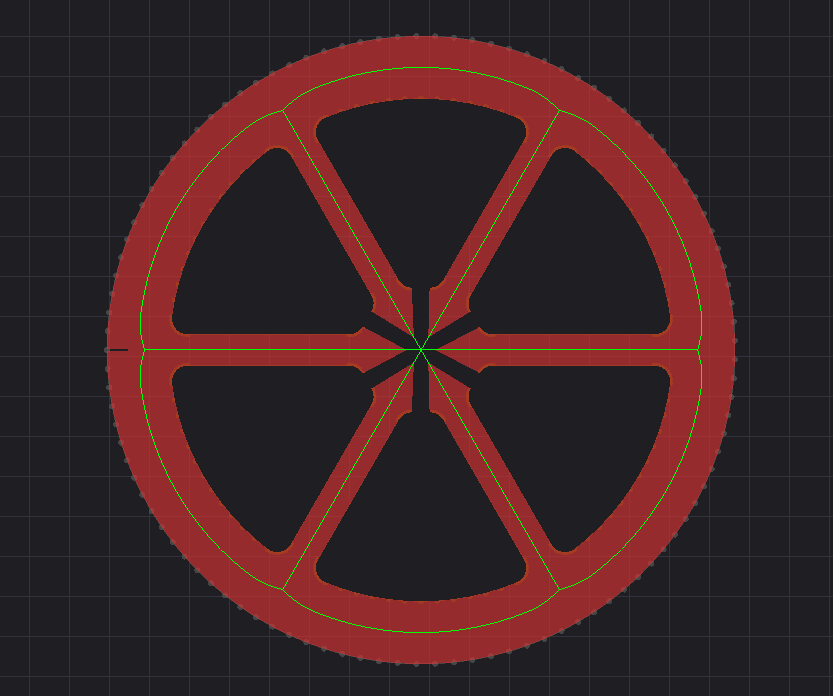
\includegraphics[width=\linewidth]{imgs/roda_pj3.png}
        \caption{Merged Thin Walls with \textit{threshold $T_3>T_2$}}
    \end{subfigure}
    
    \caption{Different thin wall scenarios for the Cogwheel}
\end{figure}

\clearpage

\clearpage
\subsection*{Cogwheel with Hole}
\vspace*{\fill}
\begin{figure}[H]
    \centering
    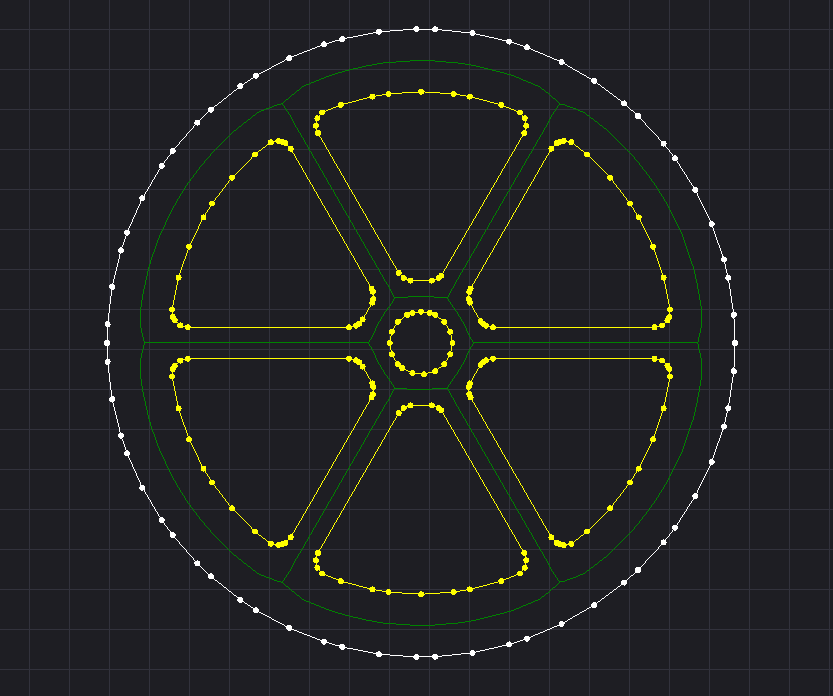
\includegraphics[width=0.85\textwidth]{imgs/rodaf.png} 
    \caption{Polygon for the Cogwheel with Hole}
\end{figure}
\vspace*{\fill}
\clearpage

\begin{figure}[H]
    \centering
    \begin{subfigure}{0.48\textwidth}
        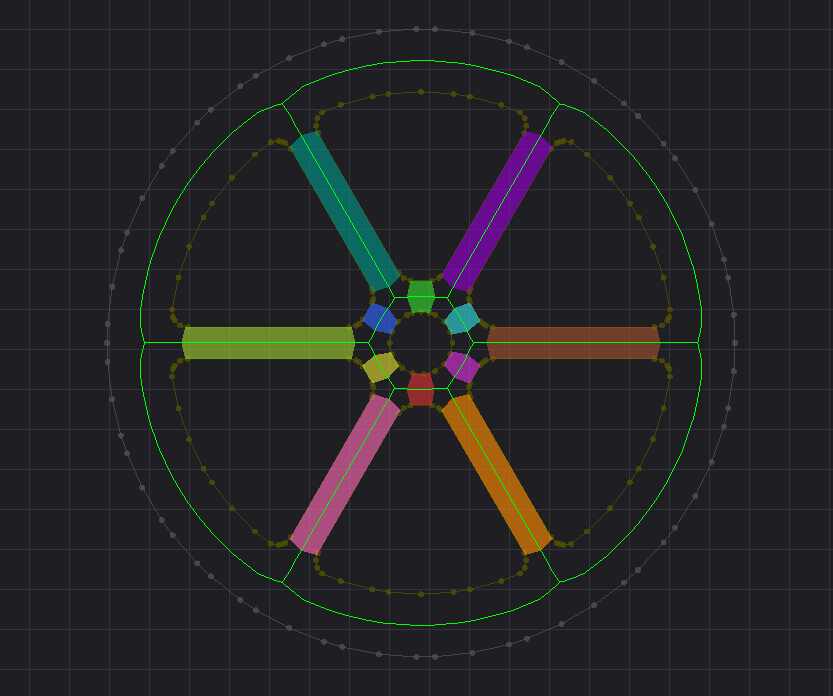
\includegraphics[width=\linewidth]{imgs/rodaf_ps.png}
        \caption{Thin Walls in groups with \textit{threshold $T_1$}}
    \end{subfigure}\hfill
    \begin{subfigure}{0.48\textwidth}
        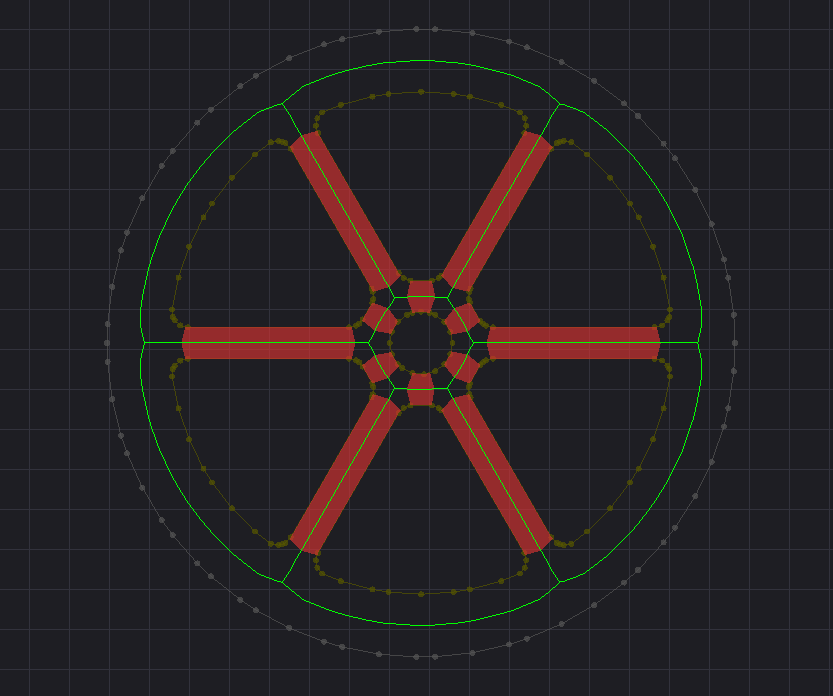
\includegraphics[width=\linewidth]{imgs/rodaf_pj.png}
        \caption{Merged Thin Walls with \textit{threshold $T_1$}}
    \end{subfigure}
    
    \vspace{0.3cm}
    
    \begin{subfigure}{0.48\textwidth}
        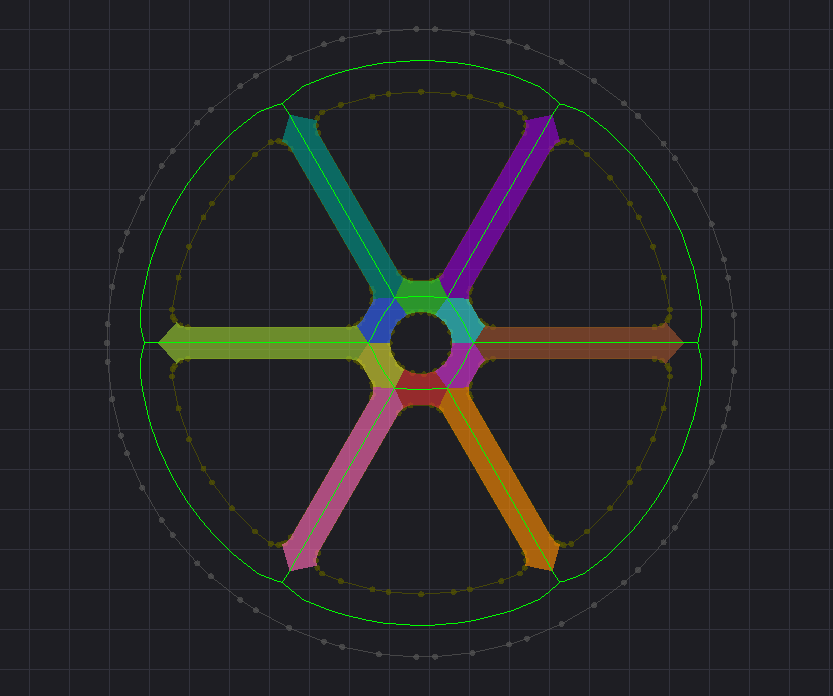
\includegraphics[width=\linewidth]{imgs/rodaf_ps2.png}
        \caption{Thin Walls in groups with \textit{threshold $T_2>T_1$}}
    \end{subfigure}\hfill
    \begin{subfigure}{0.48\textwidth}
        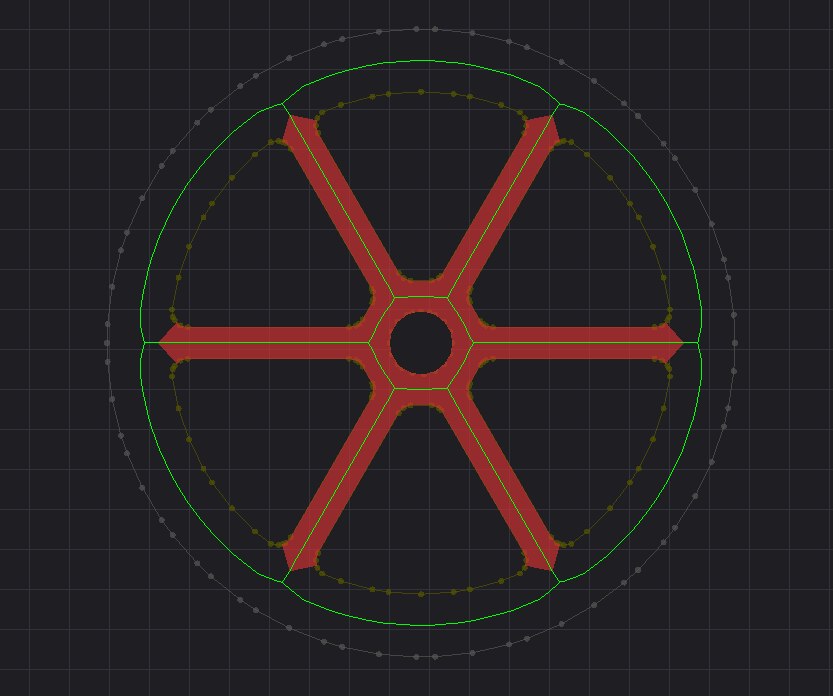
\includegraphics[width=\linewidth]{imgs/rodaf_pj2.png}
        \caption{Merged Thin Walls with \textit{threshold $T_2>T_1$}}
    \end{subfigure}
    
    \vspace{0.3cm}
    
    \begin{subfigure}{0.48\textwidth}
        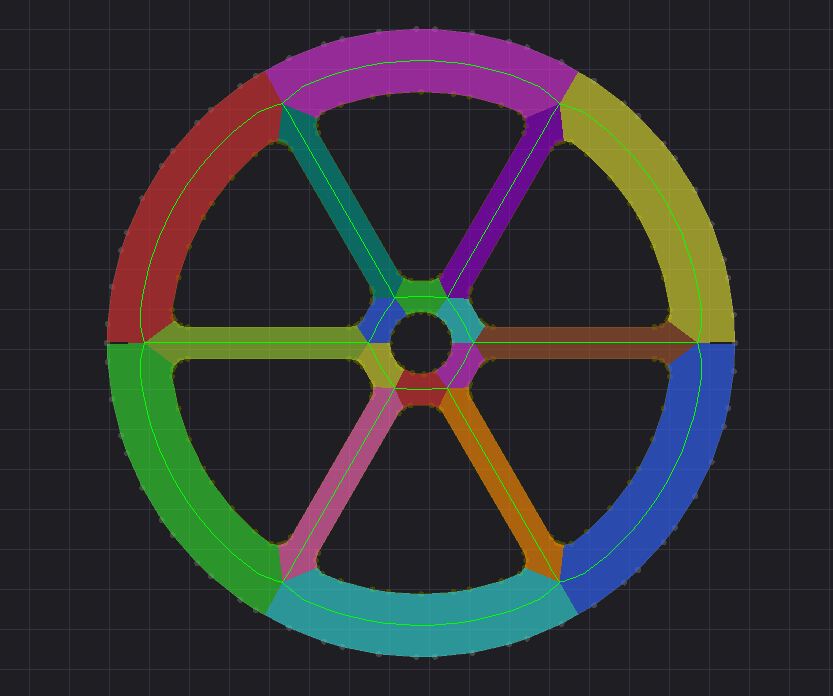
\includegraphics[width=\linewidth]{imgs/rodaf_ps3.png}
        \caption{Thin Walls in groups with \textit{threshold $T_3>T_2$}}
    \end{subfigure}\hfill
    \begin{subfigure}{0.48\textwidth}
        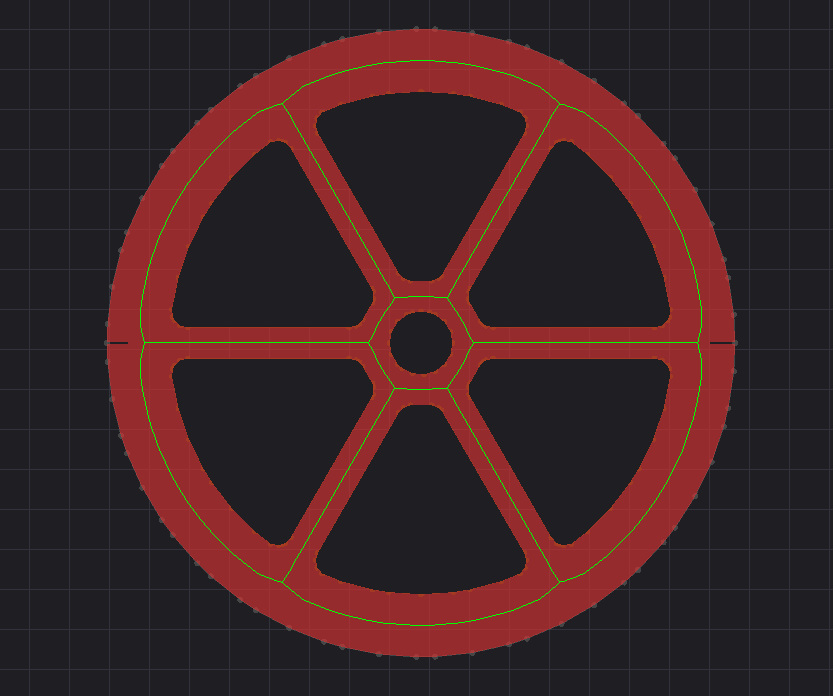
\includegraphics[width=\linewidth]{imgs/rodaf_pj3.png}
        \caption{Merged Thin Walls with \textit{threshold $T_3>T_2$}}
    \end{subfigure}
    
    \caption{Different thin wall scenarios for the Cogwheel with Hole}
\end{figure}

\clearpage

\subsection*{Miscellaneous Geometries}

\begin{figure}[H]
    \centering
     \begin{subfigure}{0.48\textwidth}
        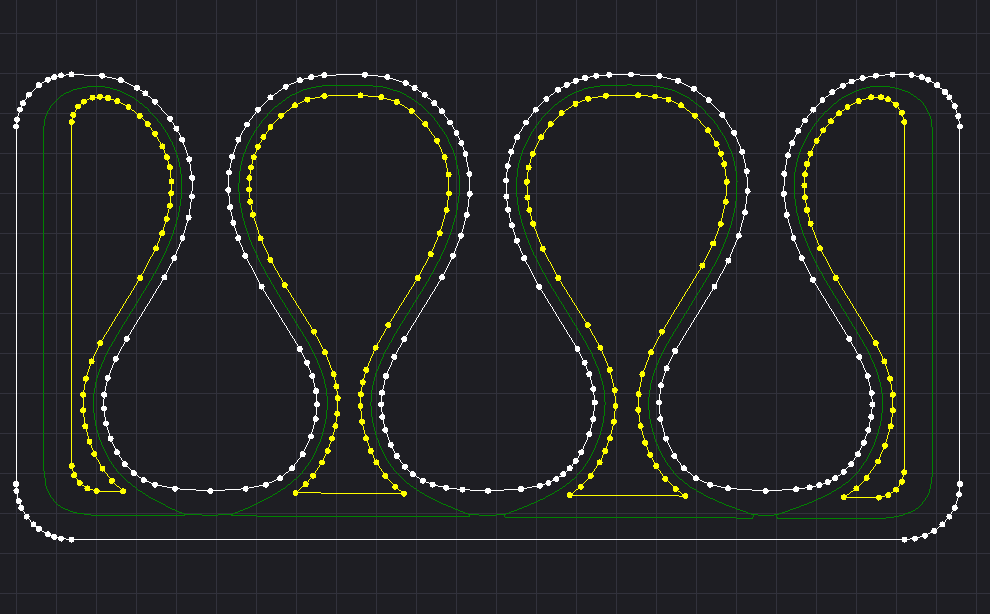
\includegraphics[width=\linewidth]{imgs/geo1.png}
        \caption{Polygon for the Comb geometry}
    \end{subfigure}
    
    \begin{subfigure}{0.48\textwidth}
        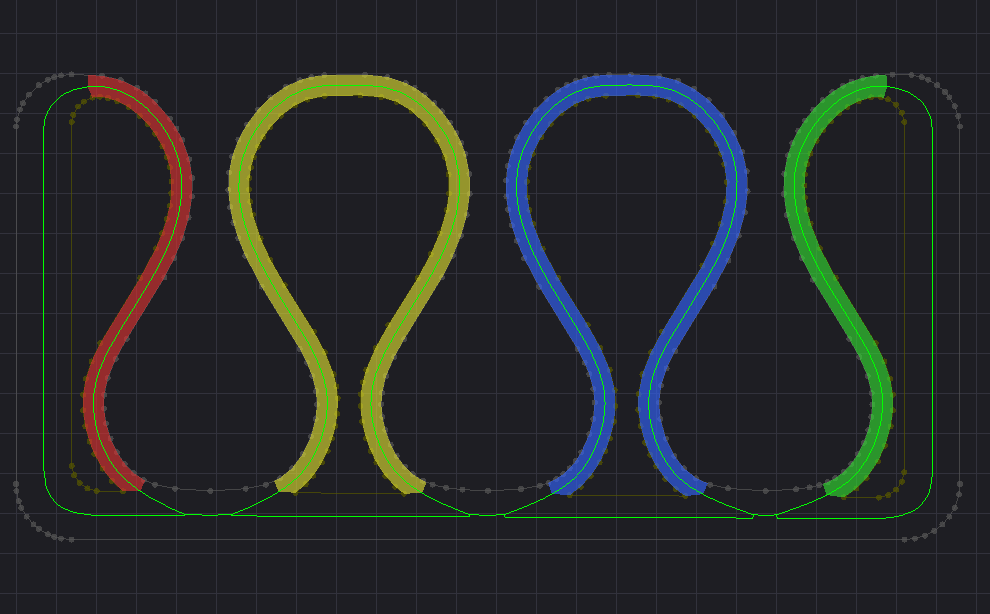
\includegraphics[width=\linewidth]{imgs/geo1_ps.png}
        \caption{Thin Walls in groups with \textit{threshold $T$}}
    \end{subfigure}\hfill
    \begin{subfigure}{0.48\textwidth}
        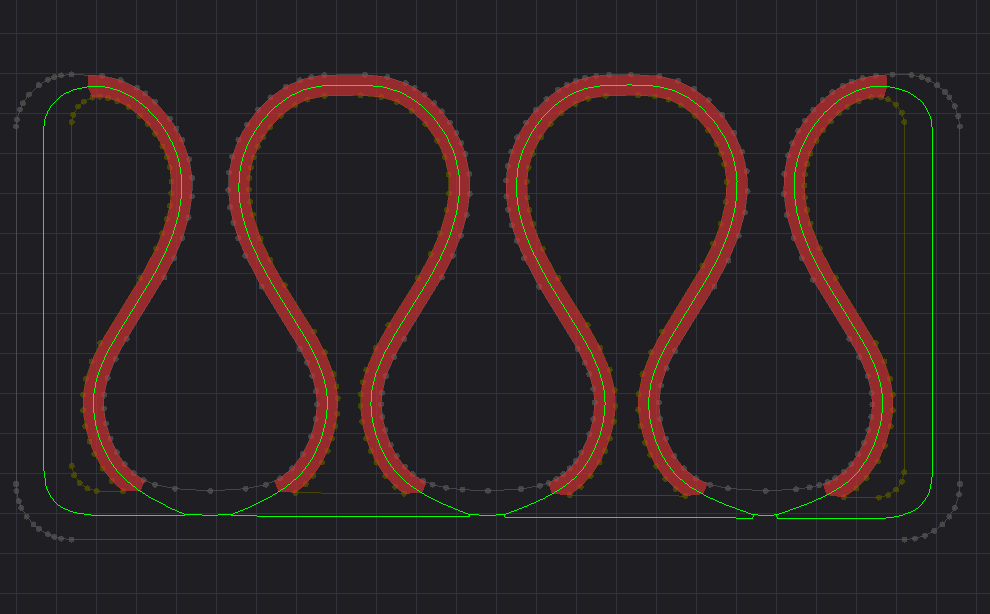
\includegraphics[width=\linewidth]{imgs/geo1_pj.png}
        \caption{Merged Thin Walls with \textit{threshold $T$}}
    \end{subfigure}
    
    \caption{Thin Walls for Comb}
\end{figure}

%\subsection*{Maze}

\begin{figure}[H]
    \centering
     \begin{subfigure}{0.48\textwidth}
        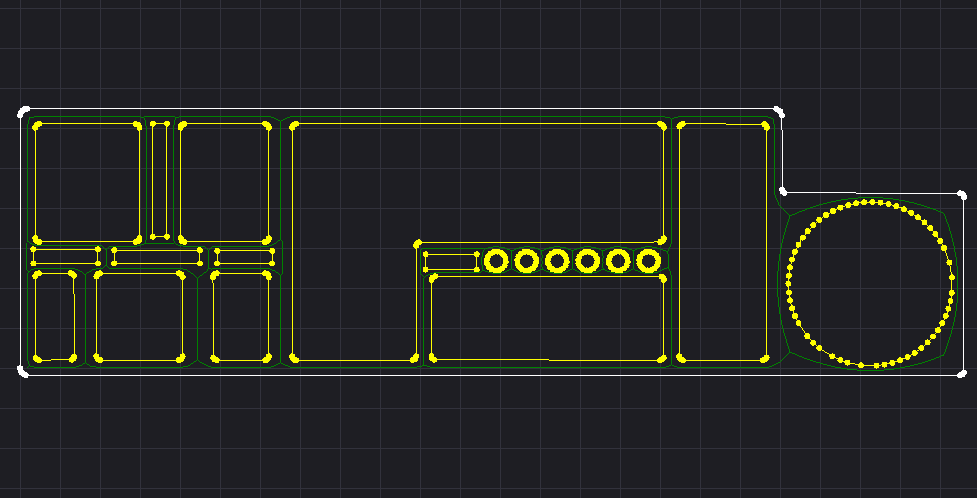
\includegraphics[width=\linewidth]{imgs/geo4.png}
        \caption{Polygon for the Maze geometry}
    \end{subfigure}
    
    \begin{subfigure}{0.48\textwidth}
        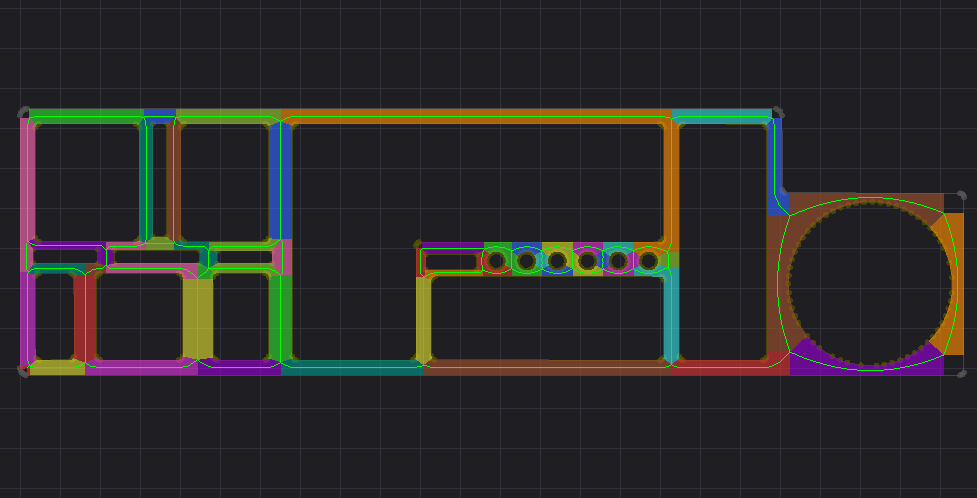
\includegraphics[width=\linewidth]{imgs/geo4_ps.png}
        \caption{Thin Walls in groups with \textit{threshold $T$}}
    \end{subfigure}\hfill
    \begin{subfigure}{0.48\textwidth}
        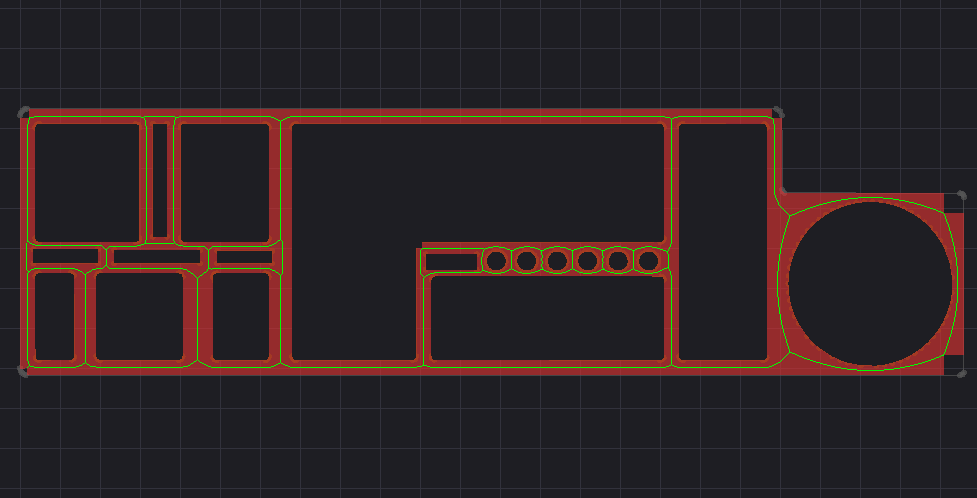
\includegraphics[width=\linewidth]{imgs/geo4_pj.png}
        \caption{Merged Thin Walls with \textit{threshold $T$}}
    \end{subfigure}
    
    \caption{Thin Walls for Maze}
\end{figure}

\clearpage

\begin{figure}
    \centering
    \begin{subfigure}{0.48\textwidth}
        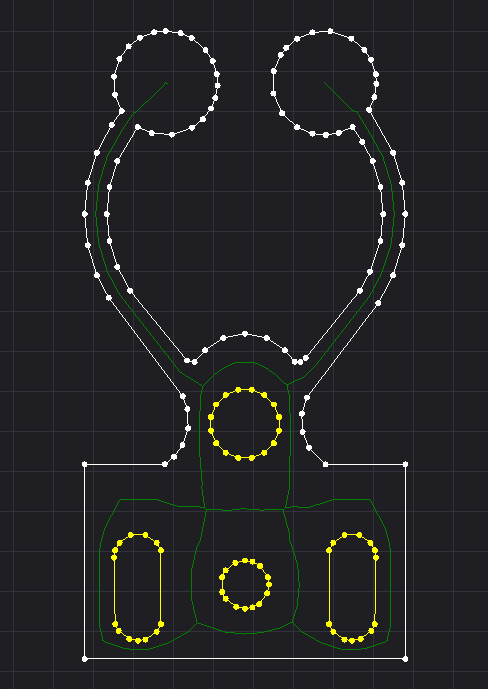
\includegraphics[width=\linewidth]{imgs/geo2.png}
        \caption{Polygon for the Tweezers geometry}
    \end{subfigure}
    
    \vspace{0.3cm}
    
    \begin{subfigure}{0.48\textwidth}
        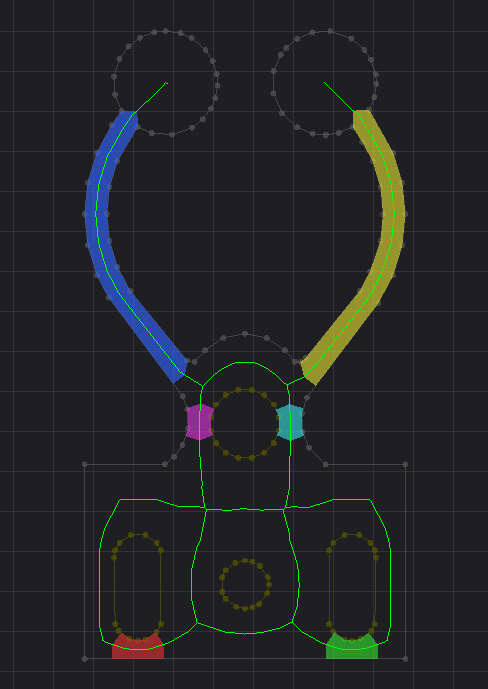
\includegraphics[width=\linewidth]{imgs/geo2_ps.png}
        \caption{Thin Walls in groups with \textit{threshold $T$}}
    \end{subfigure}\hfill
    \begin{subfigure}{0.48\textwidth}
        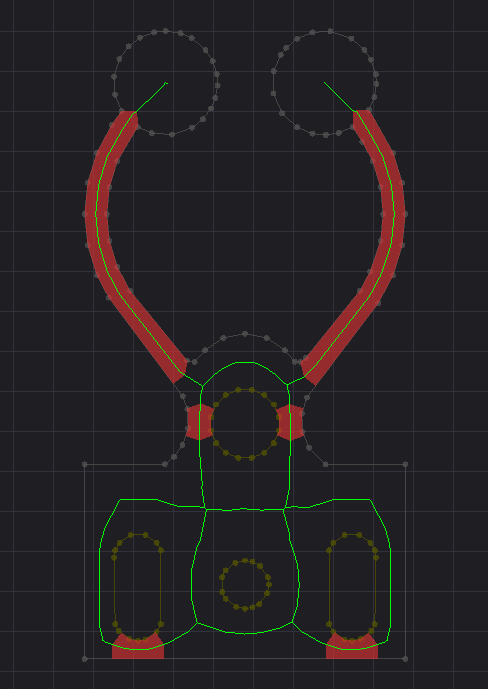
\includegraphics[width=\linewidth]{imgs/geo2_pj.png}
        \caption{Merged Thin Walls with \textit{threshold $T$}}
    \end{subfigure}
    
    \caption{Thin Walls for Tweezers}
\end{figure}

%\clearpage

\begin{figure}
    \centering
    \begin{subfigure}{0.48\textwidth}
        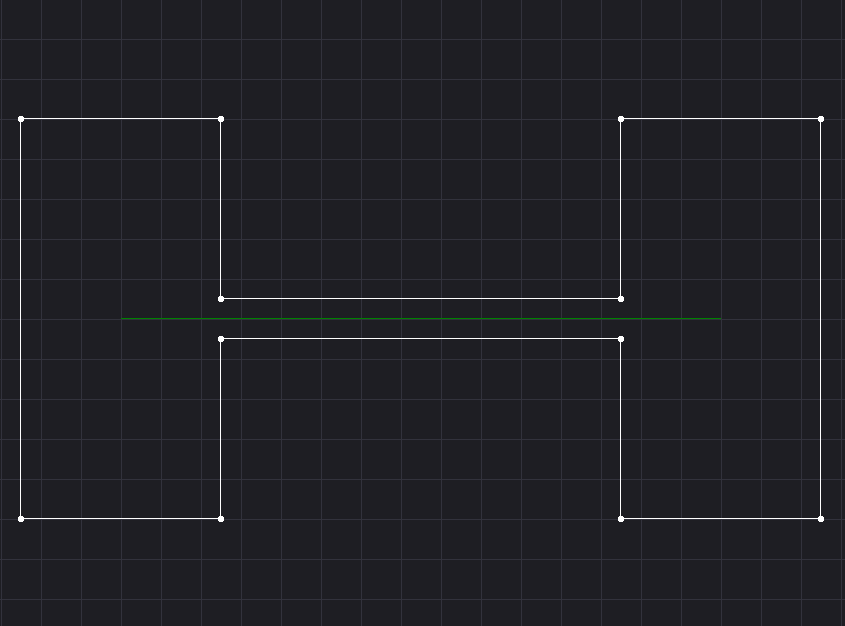
\includegraphics[width=\linewidth]{imgs/altere.png}
        \caption{Polygon for the dumbbell geometry}
    \end{subfigure}\hfill
    \begin{subfigure}{0.48\textwidth}
        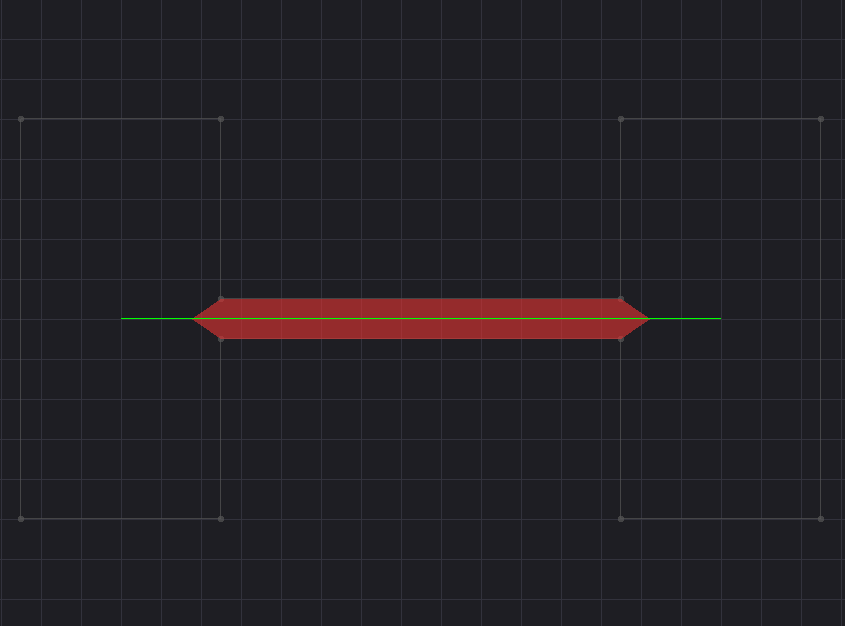
\includegraphics[width=\linewidth]{imgs/altere_pj.png}
        \caption{Thin Wall polygon of the dumbbell with \textit{threshold $T$}}
    \end{subfigure}

    \caption{Thin Walls for dumbbell}
\end{figure}

\begin{figure}
    \centering
    \begin{subfigure}{0.48\textwidth}
        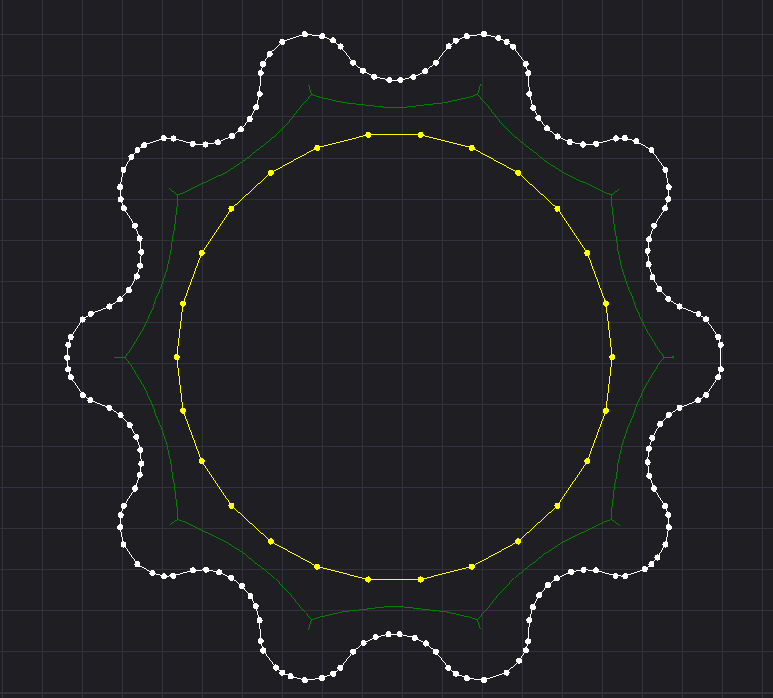
\includegraphics[width=\linewidth]{imgs/geo3.png}
        \caption{Polygon for the Gear geometry}
    \end{subfigure}
    
    \vspace{0.3cm}
    
    \begin{subfigure}{0.48\textwidth}
        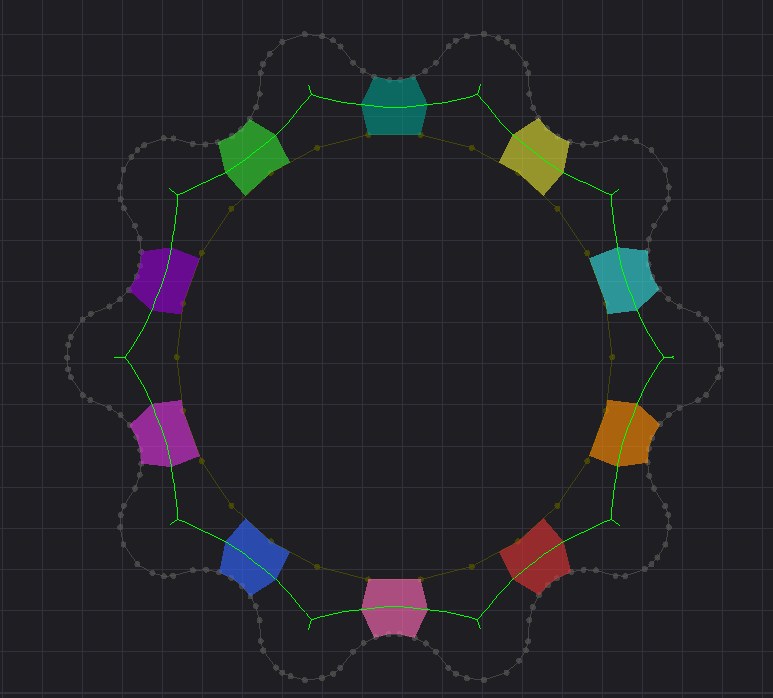
\includegraphics[width=\linewidth]{imgs/geo3_ps.png}
        \caption{Thin Walls in groups with \textit{threshold $T$}}
    \end{subfigure}\hfill
    \begin{subfigure}{0.48\textwidth}
        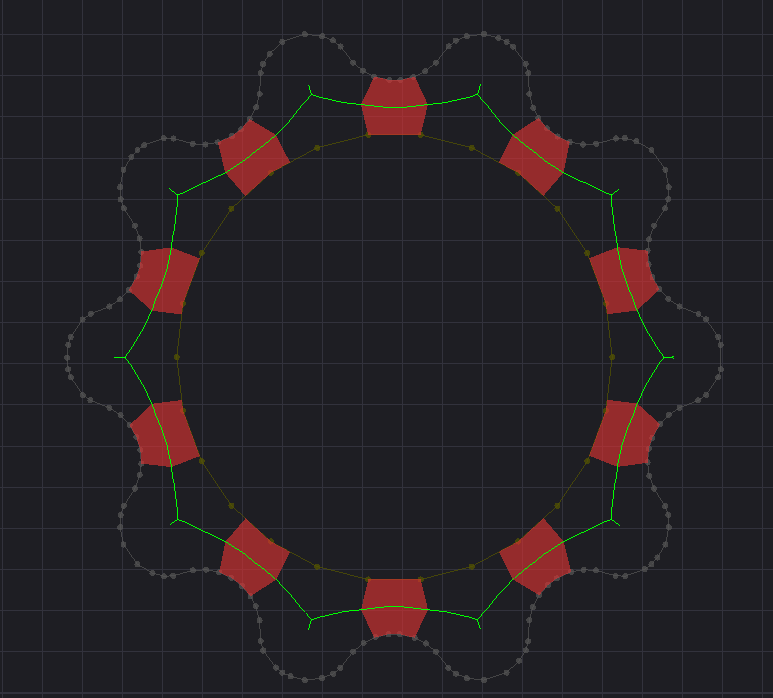
\includegraphics[width=\linewidth]{imgs/geo3_pj.png}
        \caption{Merged Thin Walls with \textit{threshold $T$}}
    \end{subfigure}
    
    \caption{Thin Walls for Gear}
\end{figure}



\end{document}
